% Bagian Tugas Pendahuluan
\section*{Tugas Pendahuluan}
\begin{enumerate}
  \item Install Fusion 360 pada Laptop masing-masing anggota kelompok \\
  \begin{figure}[H]
    \centering
    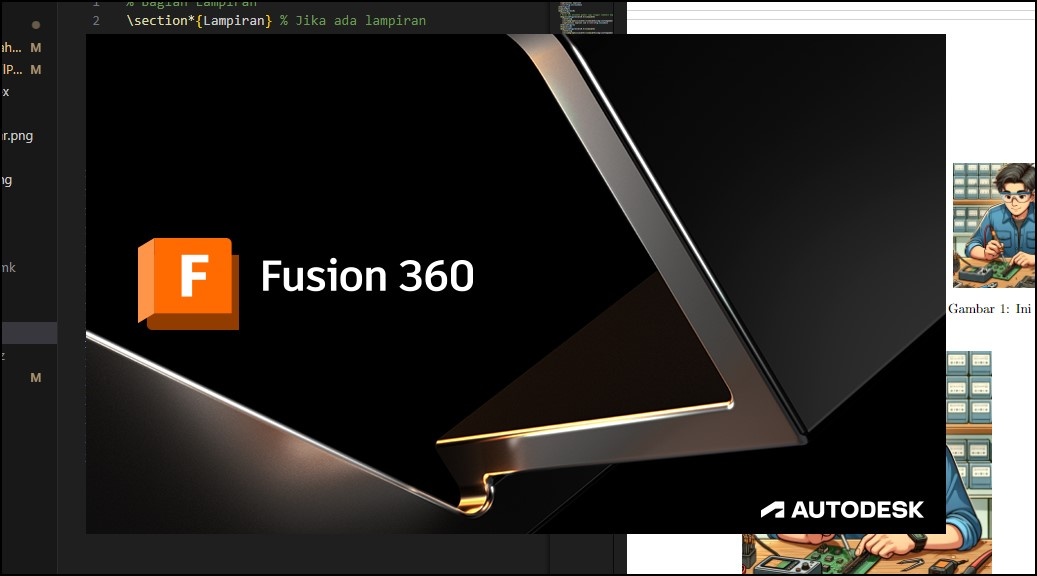
\includegraphics[width=0.6\linewidth]{img/buktidownloadfusion360.jpg}
    \caption{Bukti download FUSION 360} 
  \end{figure}
  \item Buat jalur PCB rangkaian regulator lm7805 dari schematic yang telah disediakan
  pada folder praktikan \\
  \begin{figure}[H]
    \centering
    % Kalau mau menambah gambar lagi tinggal nambahin begin{subfigure} -> end{subfigure}
    \begin{subfigure}[b]{0.45\linewidth}
      \centering
      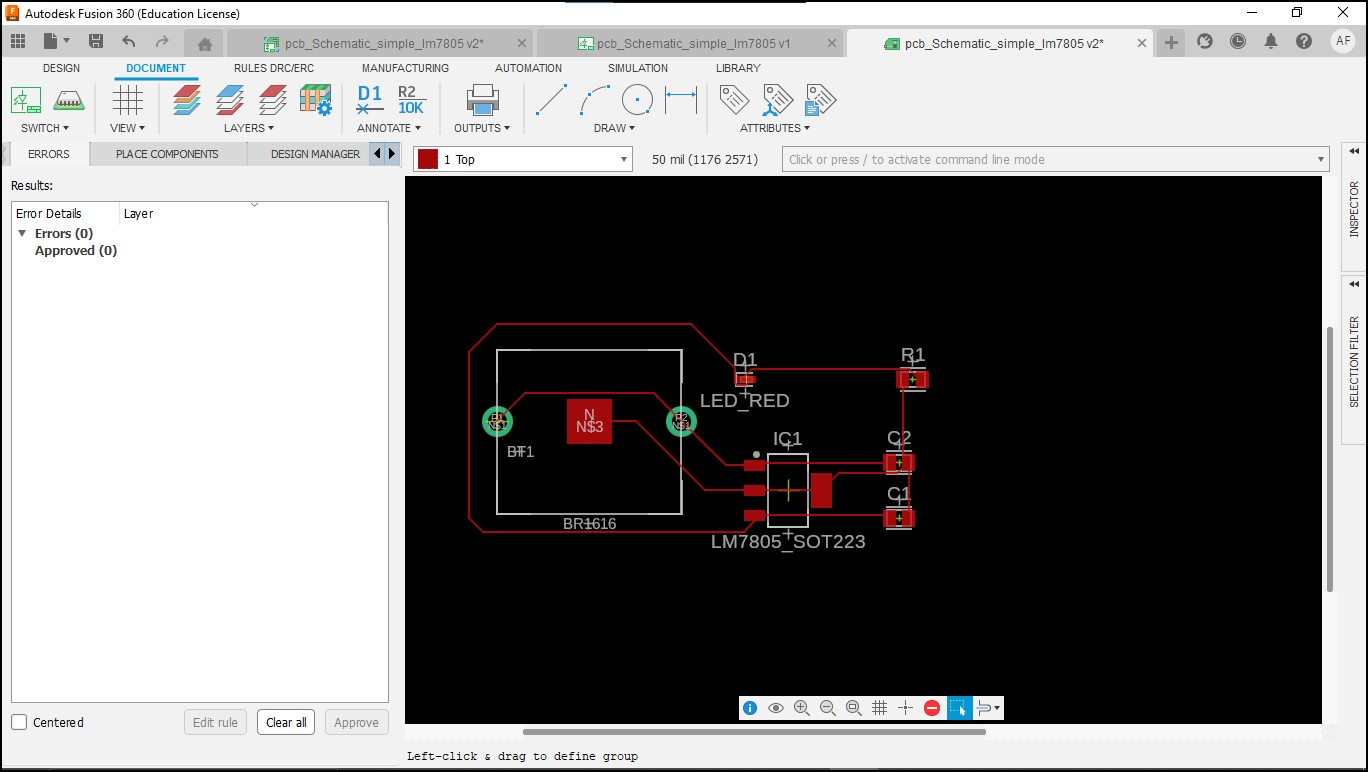
\includegraphics[width=\linewidth]{img/buatpcb.jpg}
      \caption{Bukti desain PCB\label{fig:inisub1}}
    \end{subfigure}
    \hspace{1cm}
    \begin{subfigure}[b]{0.45\linewidth}
      \centering
      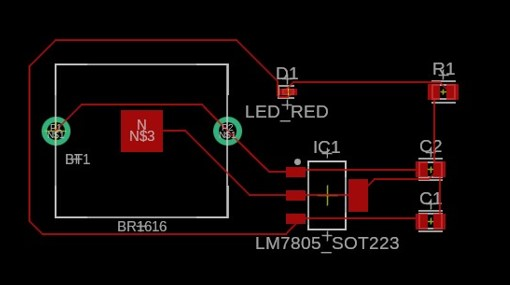
\includegraphics[width=\linewidth]{img/buatpcb(2).jpg}
      \caption{Jalur PCB\label{fig:inisub2}}
    \end{subfigure}
    \caption{Membuat jalur PCB rangkaian regulator lm7805 dari schematic yang telah disediakan\label{fig:keduagambar}}
  \end{figure}
\end{enumerate}